\documentclass[a4paper]{ctexart}

\usepackage{amsmath}
\usepackage{amssymb}
\usepackage[UTF8, scheme=plain]{ctex}
\usepackage{fancyhdr}
\usepackage{gensymb}
\usepackage[margin=1in]{geometry}
\usepackage{hyperref}
\usepackage{indentfirst} % 首行缩进
\usepackage{lastpage}
\usepackage{ragged2e}
\usepackage{tikz}
\usepackage{upgreek}
\usepackage{verbatim}
\usepackage{xassoccnt}

\usetikzlibrary{calc}

\date{} % not display time here

\fancyhf{}
\pagestyle{fancy} %fancyhdr宏包新增的页面风格

\begin{document}
    % whether show solutions 
    \newif\ifshowSolution
    % \showSolutiontrue
    \showSolutionfalse

    % 不显示自动编号 且 能自动生成目录
    \setcounter{secnumdepth}{0}
    % 行距
    \renewcommand{\baselinestretch}{1.5}

    \title{\heiti\zihao{2} 张煜曼数学错题集}
    \maketitle
    \thispagestyle{empty} % 标题页不显示页码
    \centerline{开始时间:}
    \centerline{结束时间:}

    \vfill
    \centerline{\date{\today}}

    \setlength{\parindent}{2em}
    \newpage

    % 目录 罗马数字页码
    \setcounter{page}{1}
    \pagenumbering{Roman}
    \cfoot{\thepage}

    % foot decorative lines
    % \renewcommand{\footrulewidth}{1pt}
    % \fancyhead[R]{\textbf{《鲁迅全集》笔记}}

    \hypersetup{colorlinks=true, linktocpage=true}
    \tableofcontents

    % 正文 阿拉伯数字页码
    \newpage
    \setcounter{page}{1}
    \pagenumbering{arabic}
    % 当前页 of 总页数
    \cfoot{Page \thepage\ of \pageref{LastPage}}

    \zihao{4}

    \begin{sloppy}
        \begin{enumerate}
            \section{幂的运算}

\begin{comment}
\item {
    当 $ x=7, y=-\frac{1}{7}$ 时, 求 $x^{4n+1}\cdot y^{4n+2}$ ($n$为整数)的值.
    \ifshowSolution
        \fangsong\zihao{4}
        \\
        思路: 观察到$xy=-1$,让将$x$和$y$凑成一对,相乘.直接将$x, y$的值代入表达式中进行计算.

        解答: 
        \begin{align*}
            \mbox{原式} &= 7^{4n+1}\cdot \left(-\frac{1}{7}\right) ^{4n+2}\\
            &= [7\times(-\frac{1}{7})]^{4n+1} \cdot(-\frac{1}{7})\\
            &= (-1)^{4n+1} \cdot(-\frac{1}{7})\\
            &= \frac{1}{7}.
        \end{align*}
    \else
        \\ \\ \\
    \fi
}
\end{comment}

\begin{comment}
\item {
    已知$ m=8^9, n=9^8 $, 用含$m, n$的式子表示 $72^{72}$.
    \ifshowSolution
        \fangsong\zihao{4}
        \\
        思路: 观察到$72=8\times 9$,将原式中的72分解,凑出$m, n$.
        
        解答: 
        \begin{align*}
            \mbox{原式} &= (8\times 9)^{72}\\
            &= 8^{72}\times 9^{72}\\
            &= (8^9)^8\times (9^8)^9\\
            &= m^8 n^9.
        \end{align*}
    \else
        \\ \\ \\
    \fi
}
\end{comment}

\begin{comment}
\item {
    已知$x-y=k$, 求$(3x-3y)^3.$
    \ifshowSolution
        \fangsong\zihao{4}
        \\
        解答: 
        \begin{align*}
            \mbox{原式} &= [3(x-y)]^3\\
            &= 27(x-y)^3\\
            &= 27k^3.
        \end{align*}
    \else
        \\ \\ \\
    \fi
}
\end{comment}

\begin{comment}
\item {
    若$(a^nb^mb)^3 = a^9 b^{15}$, 求$2^{m+n}$.
    \ifshowSolution
        \fangsong\zihao{4}
        \\
        思路: 先将左边化简,再与右边比较,解出$m,n$.
        
        解答: 
        \begin{align*}
            (a^nb^{m+1})^3 &= a^9b^{15}\\
            a^{3n}b^{3m+3} &= a^9b^{15}
        \end{align*}
        $\therefore 3n=9, 3m+3=15$\\
        $\therefore n=3, m=4$
        \begin{align*}
            2^{m+n} &= 2^7\\
            &= 128.
        \end{align*}
    \else
        \\ \\ \\
    \fi
}
\end{comment}

\begin{comment}
    \item {
        化简: $(-a-b)^{2n}$ ($n$为整数).
    }
    \\ \\ \\
    \item {
        化简: $(-a-b)^{2n+1}$ ($n$为整数).
    }
    \\ \\ \\

    \item {
        (用科学计数法表示)已知 1 nm = 0.000000001 m, 则 15 nm 等于多少 m?
        \ifshowSolution
        \fangsong\zihao{4}
        \\
        解答: 

        \textcircled{1} 写出换算关系
        \begin{align*}
            1 \rm{nm} &= 10^{-9} \rm{m}
        \end{align*}
        \textcircled{2} 两边同时乘15
        \begin{align*}
            15 \rm{nm} &= 15 \times 10^{-9} \rm{m}\\
            &= 1.5\times 10^{-8} \rm{m}.
        \end{align*}
        \fi
    }
    \\ \\ \\

    \item {
        (用科学计数法表示)肥皂泡表面厚度大约是 0.0007 mm,换算成以米为单位是多少?
    \ifshowSolution
    \fangsong\zihao{4}
    \\
    解答: 

    \textcircled{1} 写出换算关系
    \begin{align*}
        1 \rm{mm} &= 10^{-3} \rm{m}
    \end{align*}
    \textcircled{2} 两边同时乘0.0007
    \begin{align*}
        0.0007 \rm{mm} &= 0.0007 \times 10^{-3} \rm{m}\\
        &= 7\times 10^{-7} \rm{m}.
    \end{align*}
    \fi
    }
    \\ \\ \\
\end{comment}

\begin{comment}
\item {
    (用科学计数法表示)已知 $0.25 \upmu$m $ = 2.5\times 10^{-7}$m,那么 1 m 等于多少$\upmu$m?
    \ifshowSolution
        \fangsong\zihao{4}
        \\
        思路: 将题中给出的换算关系两边同时除以 $2.5\times 10^{-7}$,右边就出现了 1m.

        解答: 
        \begin{align*}
            \frac{0.25}{2.5\times 10^{-7}} \rm{\upmu m} &= 1\rm{m}\\
            \frac{2.5\times 0.1}{2.5\times \frac{1}{10^7}} \rm{\upmu m} &= 1\rm{m}\\
            0.1\times 10^7 \rm{\upmu m} &= 1\rm{m}\\
            10^6 \rm{\upmu m} &= 1\rm{m}\\
            1\rm{m} &= 10^6 \rm{\upmu m}.
        \end{align*}
    \else
        \\ \\ \\
    \fi
}
\end{comment}

\begin{comment}
    \item {
        若多项式$ 9x^2 - mx+16$是一个完全平方式,则 $m$的值是多少?
    }
    \\ \\ \\
\end{comment}

\begin{comment}
\item {
    已知$a^2+b^2=8, a-b=3$,求$ab$的值.
    \ifshowSolution
        \fangsong\zihao{4}
        \\
        思路: 看到$a^2+b^2, a-b, ab$, 应该想到完全平方公式.
    \else
        \\ \\ \\
    \fi
}
\end{comment}

\begin{comment}
    \item {
        若$x^2+mx+9$是完全平方式,求常数$m$的值.
    }
    \\ \\ \\

    \item {
        若$x+y=2$,求代数式$x^2-y^2+4y$的值.
    }
    \\ \\ \\
\end{comment}



\begin{comment}
\item {
    (注意: 除号使用分数形式) 已知$10^{-m}=a, 10^{-n}=b$($m, n$是整数),求$10^{2m-3n}$的值(用含有$a, b$的代数式表示).
    \\ \\ \\
}
\end{comment}

\begin{comment}
\item {
    已知$2^x=3, 2^y=6, 2^z=12$,判断下列有关$x, y, z$的数量关系式的对错.\\
    (1) $x+z=2y$\\
    (2) $x+y+3=2z$\\
    (3) $4x=z$\\
    (4) $x+1=y$
    \\ \\
}
\end{comment}

\item {
    计算: $ (\frac{1}{2})^{-1} + \lvert 2-\pi \rvert $
    \ifshowSolution
    \fangsong\zihao{4}
    \\
    思路: 去绝对值符号,运算到底.

    解答: 
    \begin{align*}
        \mbox{原式} &= 2 + \pi - 2\\
        &= \pi.
    \end{align*}
    \else
        \\ \\ \\
    \fi
}

\begin{comment}
\item {
    已知$(x+2)^{x+5}=1$, 求$x$.
    \\ \\ \\
}
\end{comment}

\item {
    $\bigstar$
    (用科学记数法)一个正方体集装箱的棱长为 $0.8 \rm{m}$.\\
    % (1) 这个集装箱的体积是多少?(用科学记数法)\\
    (2) 若有一个小立方块的棱长为$2\times 10^{-3} $ m, 则需要多少个这样的小立方块才能将集装箱装满?
    \ifshowSolution
    \fangsong\zihao{4}
    \\
    思路: 问题(2)注意简便运算.

    解答:
    \begin{align*}
        \frac{0.8^3} {(2\times 10^{-3})^3} &= \frac{0.8^3} {8\times 10^{-9}}\\
        &= \frac{0.064} {\frac{1}{10^9}}\\
        &= 0.064\times 10^9\\
        &= 6.4\times 10^{-2}\times 10^9\\
        &= 6.4\times 10^7\\
    \end{align*}
    \else
        \\ \\ \\
    \fi
}

\begin{comment}
    \item {
        (把 $\frac{1}{27}$ 化为以3为底的幂) 若$3^{x-1}=\frac{1}{27}$, 求$x$.
        \\ \\ \\
    }
\end{comment}
    
\begin{comment}
\item {
    (注意: 除号使用分数形式) 已知$a^{2n}=3, a^{3m}=5$, 求$a^{6n-9m}$.
    \ifshowSolution
    \fangsong\zihao{4}
    \\
    思路: 将$a^{6n-9m}$凑出$a^{2n}, a^{3m}$, 直接代入计算. 结果使用分数形式即可.

    解答: 
    \begin{align*}
        a^{6n-9m} &= \frac{a^{6n}}{a^{9m}}\\
        &= \frac{(a^{2n})^3} {(a^{3m})^3}\\
        &= \frac{3^3} {5^3}\\
        &= \frac{27} {125}.
    \end{align*}
    \else
        \\ \\ \\
    \fi
}
\end{comment}

\begin{comment}
    \item {
        已知$3\cdot2^x + 2^{x+1}=40$, 求$x$.
        \ifshowSolution
        \fangsong\zihao{4}
        \\
        思路: 将左边的2个$2^{x}$整理到一起.
    
        解答: 
        \begin{align*}
            3\cdot2^x + 2^{x+1} &= 40\\
            3\cdot2^x + 2\cdot 2^{x} &= 40\\
            5\cdot2^x &= 40\\
            2^x &= 8\\
            \therefore x = 3.
        \end{align*}
        \else
            \\ \\ \\
        \fi
    }
\end{comment}
            % \section{整式乘法}

\item {
    (用2种方法)若把代数式$x^2-4x-5$化成$(x-m)^2+k$的形式,其中$m,k$为常数. 求$m+k$的值.
    \ifshowSolution
        \fangsong\zihao{4}
        \\
        思路1: 把$x^2-4x-5$转化为$(x-m)^2+k$的形式, 求出m和k.

        解答: 
        \begin{align*}
            x^2-4x-5 &= x^2 - 2\times 2x + 4 - 9 \\
            &= (x-2)^2 - 9 \\
        \end{align*}
        所以,
        \[\left\{ 
            \begin{array}{lc}
                m = 2\\
                k =-9
            \end{array}
        \right.\]
        $\therefore m+k=-7.$
    \else
        \\ \\ \\
    \fi
}

\item {
    用公式计算: $(x+2y-3z)^2$.
    \\ \\ \\
}

\begin{comment}
\item {
    $a=2^{44}, b=3^{33}, c=5^{22}$, 比较$a, b, c$的大小.
    \ifshowSolution
    \fangsong\zihao{4}
    \\
    思路: 把指数化为一样,比较底数大小.

    解答: 
    \begin{align*}
        a &= (2^4)^{11} = 16^{11}\\
        b &= (3^3)^{11} = 27^{11}\\
        c &= (5^2)^{11} = 25^{11}\\
        & 16^{11} < 25^{11} < 27^{11}\\
        &\therefore a < c < b.
    \end{align*}
    \else
        \\ \\ \\
    \fi
}
\end{comment}

\begin{comment}
\item {
    已知$100^a=20, 1000^b=50$, 则$a+\frac{3}{2}b-\frac{3}{2}$的值是多少?
    \ifshowSolution
    \fangsong\zihao{4}
    \\
    思路: 观察$100^a, 1000^b$ 发现 $a,b$都出现在指数上, 要求$a+\frac{3}{2}b-\frac{3}{2}$的值, 应该想到尝试把$a+\frac{3}{2}b-\frac{3}{2}$放在指数上.

    解答: 
    \begin{align*}
        100^{a+\frac{3}{2}b-\frac{3}{2}} &= \frac{100^a\cdot 100^{\frac{3}{2}b}}{100^\frac{3}{2}}\\
        &= \frac{100^a\cdot 10^{2\cdot \frac{3}{2}b}}{10^{2\cdot\frac{3}{2}}}\\
        &= \frac{100^a\cdot 10^{3b}} {10^{3}}\\
        &= \frac{100^a\cdot 1000^{b}} {1000}\\
        &= \frac{20\times 50} {1000}\\
        &= 1\\
        &\therefore a+\frac{3}{2}b-\frac{3}{2} = 0.
    \end{align*}
    \else
        \\ \\ \\
    \fi
}
\end{comment}

\item {
    用多项式乘法法则推导完全平方公式.
}
\\ \\ \\

\item {
    计算 $(-x-y)^2$.
    \ifshowSolution
    \fangsong\zihao{4}
    \\
    思路: 先将括号里的负号处理掉, 再用公式.

    解答: 
    \begin{align*}
        \mbox{原式} &= (x+y)^2\\
        &= x^2 +2xy + y^2
    \end{align*}
    \else
        \\ \\ \\
    \fi
}

\item {
    判断下列各式的正误.

    \textcircled{1}$(a-b)^2 = a^2 - b^2$\\
    \textcircled{2}$(-2a-3b)^2 = 4a^2 - 12ab +9b^2$\\
    \textcircled{3}$(\frac13 m + \frac12 n)^2 = \frac19 m^2 + \frac16 mn + \frac14 n^2$\\
    \textcircled{4}$(-y-3)^2 = y^2 + 6y + 9$
    \\ \\ \\
}

\item {
    用公式计算.

    $(1) (-\frac34 x + \frac43 y)^2$ \\ \\

    $(2) (-7m-2n)^2$ \\ \\
    
    $(3) (a+b+c)^2$ \\ \\
}
\\ \\

\item {
    多项式 $a^2 + 4$ 加上一个单项式后, 可化为一个多项式的平方, 求这个单项式.(列出所有结果)
    \ifshowSolution
    \fangsong\zihao{4}
    \\
    思路: 想到完全平方公式 $(x\pm y)^2 = x^2 \pm 2xy + y^2$.

    解答: 

    (1) $a^2$对应公式里的$x^2$, $4$对应公式里的$y^2$, 所以$x= \pm a, y= \pm 2$, 所以$2xy = \pm 4a$. 即
    \begin{align*}
        (a+2)^2 = a^2 + 4a + 4 \\
        (a-2)^2 = a^2 - 4a + 4
    \end{align*}
    (2) $4$对应公式里的$x^2$, $a^2$对应公式里的$2xy$, 所以$x= \pm 2, y=\pm \frac{a^2}{4}$, 所以$y^2 = \frac{a^4}{16}$. 即
    \begin{align*}
        (2 + \frac{a^2}{4})^2 = 4 + a^2 + \frac{a^4}{16}
    \end{align*}
    \else
        \\ \\ \\
    \fi
}

\item {
    计算: $(-xy^2)\cdot (x^2y - 6xy)$
}
\\ \\ \\

\item {
    计算: $(a+3)(a-1) + a(a-2)$
}
\\ \\ \\

\item {
    计算(用公式): $(x+2y-1)\cdot (x+2y+1)$
}
\\ \\ \\

\item {
    观察下列各式, 写出第n个等式.

    第\textcircled{1}个等式: $1\times 5 + 4 = 3^2;$ \\
    第\textcircled{2}个等式: $3\times 7 + 4 = 5^2;$ \\
    第\textcircled{3}个等式: $5\times 9 + 4 = 7^2; \\ \cdots $ \\
    \ifshowSolution
        \fangsong\zihao{4}
        \\
        思路: 先找到等式中第1列的数字的规律, 再找下一列数的规律, 最后写出公式. 第一列数是奇数1,3,5,可以用n表示为 $2n-1$. 第二列数比第一列大4,所以是$2n+3$. 依此类推.

        解答: 

        $(2n-1)\times (2n+3) + 4 = (2n+1)^2$.
    \else
        \\ \\ \\
    \fi
}

\item {
    已知多项式 $x-2a$ 与 $x^2+x-1$ 的乘积中不含 $x^2$ 项, 则常数$a$的值是多少?
    \ifshowSolution
    \fangsong\zihao{4}
    \\
    思路: 不含 $x^2$ 项的意思即该项的“系数为0”.展开后合并同类项.
    \else
        \\ \\ \\
    \fi
}

\item {
    多项式 $4a^2+9$ 加上一个单项式后, 可化为一个多项式的平方, 求这个单项式.
}
\\ \\ \\

\item {
    已知 $a^2+a-1=0$, 求 $a^3 + 2a^2 + 2023$ 的值.
}
\\ \\ \\

\item {
    用公式计算: $(a-2b+3c)\cdot (a+2b+3c)$.
}
\\ \\ \\

\item {
    已知公式: $(x-1)(x^n + x^{n-1} + \cdots + x + 1) = x^{n+1} - 1$ (n为正整数).
    
    利用上述公式, 求 $2^{100} + 2^{99} +\cdots + 2^2 + 2$ 的值.
    \ifshowSolution
        \fangsong\zihao{4}
        \\
        思路: 使用公式前, 必须把原式的形式整理得和公式完全一致.
    \else
        \\ \\ \\
    \fi
}

\item {
    用若干A类正方形(边长a)、B类长方形(长a,宽b)、C类正方形(连长b),拼成一个边长为 $2a + 2b$ 的正方形,需要B类正方形多少个?
    \ifshowSolution
        \fangsong\zihao{4}
        \\
        思路: 画图.
    \else
        \\ \\ \\
    \fi
}

\item {
    观察``杨辉三角'',计算 $(a+b)^5$ 的结果中,项 $a^3b^2$的系数,
    \[
    \begin{matrix}
        & & & & 1 & & & \\
        & & & 1 & & 1 & & \\
        & & 1 & & 2 & & 1 & \\
        & 1 & & 3 & & 3 & & 1 \\
        1 & & 4 & & 6 & & 4 & & 1
    \end{matrix}
    \]
    \begin{align*}
        (a+b)^1 &= a+b \\
        (a+b)^2 &= a^2 + 2ab + b^2 \\
        (a+b)^3 &= a^3 + 3a^2b + 3ab^2 + b^3 \\
        (a+b)^4 &= a^4 + 4a^3b + 6a^2b^2 + 4ab^3 + b^4 \\
    \end{align*}
    \ifshowSolution
        \fangsong\zihao{4}
        \\
        % 思路: 画图.
    \else
        \\ \\ \\
    \fi
}

\item {
    判断 $49^8 - 14^2\times 7^{12}$ 能否被9整除,并说明理由.
    \ifshowSolution
        \fangsong\zihao{4}
        \\
        % 思路: .
    \else
        \\ \\ \\
    \fi
}

\item {
    求代数式 $y^2 +10y + 27$ 的最小值.
    \ifshowSolution
        \fangsong\zihao{4}
        \\
        思路: 将原式整理成 $(y + m)^2 + k$ 的形式; 再利用 $a \geq 0$ 的性质,计算出原式的最小值.
    \else
        \\ \\ \\
    \fi
}

\item {
    求代数式 $-m^2 + 4m + 8$ 的最值, 并判断是最大值还是最小值.
    \ifshowSolution
        \fangsong\zihao{4}
        \\
        思路: 利用 $a^2 \geq 0$ 的性质.
    \else
        \\ \\ \\
    \fi
}

\item {
    写出 $(a+b)^2, (a-b)^2, ab$ 三者之间的等量关系.
    \ifshowSolution
        \fangsong\zihao{4}
        \\
        % 思路:
    \else
        \\ \\ \\
    \fi
}

\item {
    若多项式 $2x^2 + kx - 14$ 是由整式 $x-2$ 与另一个整式 $2x+m$相乘得到的,求k的值.
    \ifshowSolution
        \fangsong\zihao{4}
        \\
        % 思路:
    \else
        \\ \\ \\
    \fi
}

\item {
    已知 $a^2 + a - 3 = 0$, 计算$(a^2 - 3)(a+1)$.
    \ifshowSolution
        \fangsong\zihao{4}
        \\
        % 思路:
    \else
        \\ \\ \\
    \fi
}

\item {
    若 $\lvert x+y-4 \rvert + (xy-3)^2 = 0$, 计算$x^2 + y^2$.
    \ifshowSolution
        \fangsong\zihao{4}
        \\
        % 思路:
    \else
        \\ \\ \\
    \fi
}

\item {
    在计算 $(ax+1)(2x+b)$时,小泉同学看错了$b$的值, 计算结果为$2x^2 + 6x + 4$; 小张同学看错了$a$ 的值,计算结果为 $4x^2+12x+5$.

    (1) 求 $a,b$.\\
    (2) 计算 $(ax+1)(2x+b)$ 的正确结果.
    \ifshowSolution
        \fangsong\zihao{4}
        \\
        思路: 小泉同学算出的a是正确的,小张同学算出的b是正确的.
    \else
        \\ \\ \\ \\ 
    \fi
}

            % \section{图形的变换}

\item {
    $\bigstar\bigstar\bigstar$
    如图, 已知线段AB, 求作等腰直角三角形, 使其斜边等于线段AB, 保留作图痕迹并证明. \\
    \par\bigskip
    \begin{tikzpicture}
        % 带端点标注的线段
        \draw[|-|] (1, 0) -- (4, 0) 
            node[left] at (1, 0) {A}
            node[right] at (4, 0) {B};
    \end{tikzpicture}
    \ifshowSolution
        \fangsong\zihao{6}
        \\
        思路: 先满足等腰, 再满足直角. 

        正解:\\
        \begin{tikzpicture}
            % 带端点标注的线段
            \coordinate (A) at (0, 0);
            \coordinate (B) at (4, 0);
            \coordinate (O) at (2, 0);
            \coordinate (P) at (2, -4);
            
            \draw[|-|] (A) -- (B) 
                node[left] at (0, 0) {A}
                node[right] at (4, 0) {B};

            \draw (A) +(283:4. 47cm) arc (283:310:4. 47cm);
            \draw (B) +(231:4. 47cm) arc (231:258:4. 47cm);

            \draw[-] (2, 1) -- (2, -5);

            \draw (O) +(258:2cm) arc (258:278:2cm);

            \coordinate (C) at (2, -2);
            \draw[-] (C) -- (A)
                node[below left] at (C) {C};
            \draw[-] (C) -- (B);

            \fill (O) circle node[above left] {$O$};
            \fill (P) circle node[below left] {$P$};
        \end{tikzpicture} \\
        证明: \\
        (1) 先证明 $\triangle ABC$ 是等腰三角形. \\
         $\because OP$ 是 AB 的垂直平分线, 点 C 在 AB 上, \\
        $\therefore AC = BC$. \\
        (2) 再证明 $\triangle ABC$ 是直角三角形.\\
        $\because OA = OC = OB$, \\
        $\therefore \angle A = \angle ACO, \angle B = \angle BOC,$ \\
        $\therefore \angle ACB = \angle A + \angle B.$ \\
        $\because$ 三角形内角为 $180^\circ, $ \\
        $\therefore \angle ACB = 90^\circ.$ \\
        所以, $\triangle ABC$ 是等腰直角三角形.

    \else
        \\ \\ \\ \\ \\
    \fi
}

\item {
    $\bigstar\bigstar$
    尺规作图. 已知$\triangle ABC$,作它的三个角的角平分线. 你有何发现?\\
    \begin{tikzpicture}[scale=1. 2]
    % 绘制角AOB
    \coordinate (A) at (2, 3);
    \coordinate (C) at (4, 0);
    \coordinate (B) at (0, 0);
    \draw (A) -- (B);
    \draw (C) -- (B);
    \draw (C) -- (A);
    % 标注点
    \fill (A) circle  node[above left] {$A$};
    \fill (B) circle  node[below left] {$B$};
    \fill (C) circle  node[below right] {$C$};
    \end{tikzpicture}
    \ifshowSolution
        \fangsong\zihao{6}
        \\
        % 思路: 
    \else
        \\ \\ \\ \\
    \fi
}

\item {
    $\bigstar$
    如图, $\angle AOB=45\degree$, 点$M, N$分别在射线$OA,OB$上,$MN=5, S_{\triangle OMN} = 15$, 点$P$是直线$MN$上的一个动点,点$P$关于$OA$的对称点为$P_1$,点$P$关于$OB$的对称点为$P_2$. 连接$OP_1, OP_2, P_1P_2$, 当点$P$在直线$MN$上运动时,则 $\triangle OP_1P_2$的面积的最小值是多少?此时点$P$ 在哪里? \\
    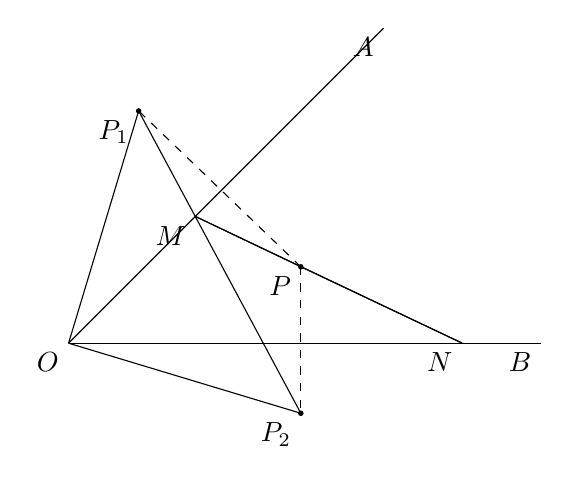
\begin{tikzpicture}[scale=1]
        % 绘制角AOB
        \coordinate (O) at (0, 0);
        \coordinate (A) at (4, 4);
        \coordinate (B) at (6, 0);
        \draw (O) -- (A);
        \draw (O) -- (B);
        
        % 标注点P
        \coordinate (P) at (2.95, 0.97);
        \coordinate (P_1) at (0.89, 2.95);
        \coordinate (P_2) at (2.95, -0.89);
        \draw [dashed] (P) -- (P_1);
        \draw [dashed] (P) -- (P_2);
        \draw (P_1) -- (P_2);
        \draw (O) -- (P_1);
        \draw (O) -- (P_2);
    
        \coordinate (M) at (1.61, 1.61);
        \coordinate (N) at (5, 0);
        \draw (M) -- (P);
        \draw (N) -- (P);
        \draw (N) -- (M);
    
        % 标注所有点
        node[left] at (0, 0) {A}
        \fill (O) circle  node[below left] {$O$};
        \fill (A) circle (0pt) node[below left] {$A$};
        \fill (B) circle (0pt) node[below left] {$B$};
        \fill (P) circle (1pt) node[below left] {$P$};
        \fill (P_1) circle (1pt) node[below left] {$P_1$};
        \fill (P_2) circle (1pt) node[below left] {$P_2$};
        \fill (M) circle (0pt) node[below left] {$M$};
        \fill (N) circle (0pt) node[below left] {$N$};
        \end{tikzpicture}
    \ifshowSolution
        \fangsong\zihao{6}
        \\
        % 思路: 18
    \else
        \\ \\ \\ \\ \\ \\
    \fi
}

\item {
    $\bigstar$
    如图,把一张长方形纸片$ABCD$沿$EF$折叠后$ED$与$BC$的交点为$G$,$D,C$分别在$M,N$的位置上,若$\angle EFG=55\degree$,则$\angle AEM$是多少度?\\
    \par\bigskip
    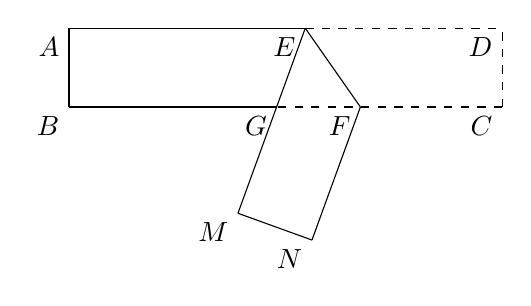
\begin{tikzpicture}[scale=0.5]
    \coordinate (A) at (-5, 1);
    \coordinate (B) at (-5, -1);
    \coordinate (C) at (6, -1);
    \coordinate (D) at (6, 1);
    \coordinate (E) at (1, 1);
    \coordinate (F) at (2.4, -1);
    \coordinate (G) at (0.27, -1);
    \coordinate (M) at (-0.71, -3.7);
    \coordinate (N) at (1.17, -4.38);

    % 画线
    \draw [dashed] (C) -- (G);
    \draw [dashed] (C) -- (D);
    \draw [dashed] (E) -- (D);
    \draw (A) -- (E);
    \draw (A) -- (B);
    \draw (G) -- (B);
    \draw (E) -- (M);
    \draw (N) -- (M);
    \draw (N) -- (F);
    \draw (E) -- (F);

    % 标注点
    \fill (A) circle (0pt) node[below left] {$A$};
    \fill (B) circle (0pt) node[below left] {$B$};
    \fill (C) circle (0pt) node[below left] {$C$};
    \fill (D) circle (0pt) node[below left] {$D$};
    \fill (E) circle (0pt) node[below left] {$E$};
    \fill (F) circle (0pt) node[below left] {$F$};
    \fill (G) circle (0pt) node[below left] {$G$};
    \fill (M) circle (0pt) node[below left] {$M$};
    \fill (N) circle (0pt) node[below left] {$N$};
    \end{tikzpicture}
    \ifshowSolution
        \fangsong\zihao{6}
        \\
        正解: $70\degree$.
    \else
        \\ \\ \\ \\
    \fi
}

\begin{comment}


\item {
    如图,是重叠的两个直角三角形。将其中一个直角三角形沿$BC$方向平移得到 $\triangle DEF$. 如果$AB=8, BE=4, DH=2$, 则图中阴影部分的面积是多少?\\
    \par\bigskip
    \begin{tikzpicture}[scale=0.3]
        \coordinate (E) at (0, 0);
        \coordinate (A) at (-4, 8);
        \coordinate (B) at (-4, 0);
        \coordinate (C) at (6, 0);
        \coordinate (D) at (0, 8);
        \coordinate (F) at (10, 0);
        \coordinate (H) at (0, 4.8);
        \draw (B) -- (A);
        \draw (D) -- (A);
        \draw (C) -- (A);
        \draw (D) -- (F);
        \draw (F) -- (B);
        \draw (D) -- (E);
        
        % 标注所有点
        \fill (A) circle (0pt) node[below left] {$A$};
        \fill (B) circle (0pt) node[below left] {$B$};
        \fill (C) circle (1pt) node[below left] {$C$};
        \fill (D) circle (1pt) node[below left] {$D$};
        \fill (E) circle (1pt) node[below left] {$E$};
        \fill (F) circle (0pt) node[below left] {$F$};
        \fill (H) circle (0pt) node[below left] {$H$};

        % 加阴影
        \pattern[pattern=horizontal lines, pattern color=gray] (D) -- (H) -- (C) -- (F);
    \end{tikzpicture}
    \ifshowSolution
        \fangsong\zihao{6}
        \\
        正解: 28.
    \else
        \\ \\ \\ \\
    \fi
}

\item {
    尺规作图. 过点$P$ 作直线$l$的垂线. \\
    \begin{tikzpicture}[scale=1. 2]
    % 绘制角AOB
    \coordinate (A) at (0, 0);
    \coordinate (C) at (4, 0);
    \coordinate (P) at (1. 5, 2);
    \draw (C) -- (A);
    % 标注点
    \fill (P) circle (2pt)  node[above left] {$P$};
    \fill (C) circle  node[below right] {$l$};
    \end{tikzpicture}
    \ifshowSolution
        \fangsong\zihao{6}
        \\
        % 思路: 
    \else
        \\ \\ \\ \\
    \fi
}

\item {
    尺规作图. 过点$P$ 作直线$l$的垂线. \\
    \par\bigskip
    \begin{tikzpicture}[scale=1. 2]
        % 绘制角AOB
        \coordinate (A) at (0, 0);
        \coordinate (C) at (4, 0);
        \coordinate (P) at (1. 5, 0);
        \draw (C) -- (A);
        % 标注点
        \fill (P) circle (2pt)  node[above left] {$P$};
        \fill (C) circle  node[below right] {$l$};
    \end{tikzpicture}
    \ifshowSolution
        \fangsong\zihao{6}
        \\
        % 思路: 
    \else
        \\ \\ \\ \\
    \fi
}

\item {
    (尺规作图)如图, 已知线段AB, 作线段AB的垂直平分线. \\
    \begin{tikzpicture}
        % 带端点标注的线段
        \draw[|-|] (0, 0) -- (4, 4) 
            node[left] at (0, 0) {A}
            node[right] at (4, 4) {B};
    \end{tikzpicture}
    \ifshowSolution
        \fangsong\zihao{6}
        \\
        % 思路: 
    \else
        \\ \\ \\ \\
    \fi
}

    \item {
        如图, $P$ 为 $\angle AOB$ 内一点, $OA$ 垂直平分线段 $PP_1$, $OB$垂直平分线段 $PP_2$, 连接$P_1P_2$ 交$OA$ 于点 $N$, 若$P_1P_2=15$, 求 $\triangle PMN$ 的周长. \\
        \begin{tikzpicture}[scale=1. 2]
        % 绘制角AOB
        \coordinate (O) at (0, 0);
        \coordinate (A) at (4, 4);
        \coordinate (B) at (4, 0);
        \draw (O) -- (A);
        \draw (O) -- (B);
        
        % 标注点P
        \coordinate (P) at (3, 2);
        \coordinate (P_1) at (2, 3);
        \coordinate (P_2) at (3, -2);
        \draw (P) -- (P_1);
        \draw (P) -- (P_2);
        \draw (P_1) -- (P_2);
    
        \coordinate (M) at (2. 17, 2. 17);
        \coordinate (N) at (2. 6, 0);
        \draw (M) -- (P);
        \draw (N) -- (P);
    
        
        % 标注所有点
        node[left] at (0, 0) {A}
        \fill (O) circle  node[below left] {$O$};
        \fill (A) circle (0pt) node[below left] {$A$};
        \fill (B) circle (0pt) node[below left] {$B$};
        \fill (P) circle (1pt) node[below left] {$P$};
        \fill (P_1) circle (1pt) node[below left] {$P_1$};
        \fill (P_2) circle (1pt) node[below left] {$P_2$};
        \fill (M) circle (0pt) node[below left] {$M$};
        \fill (N) circle (0pt) node[below left] {$N$};
        \end{tikzpicture}
        \ifshowSolution
            \fangsong\zihao{6}
            \\
            % 思路: 
        \else
            \\ \\ \\ \\
        \fi
    }
    \end{comment}
        \end{enumerate}
    \end{sloppy}
\end{document}
